\newpage
\section{Background}

Creating a web application is typically done in three steps, design, develop, and publish.

\textbf{Design:} The designer does the majority of design work at the beginning of the project. The designer and customer collaborate to create an interface until they are both satisfied.  Some developers are also present during this first part of the process to give insight into what is possible to create for the desired system.

\textbf{Develop:} Some development starts at the beginning of the project too. Generally, the development that starts at the beginning of the project is primarily functional, meaning there is no graphical interface yet. When the customer has approved the design, the development starts on the visual parts of the system. The developer takes the design and tries to mimic the design with code to which the functionality can be attached.  

\textbf{Publish:} When the web application is at the point that the customer, designer, and developers are satisfied, the application can be published. When the application is published, the customer's users have access to it. For most projects, the customer stays in touch with the designer and developers to manage the application. Management consists of fixing bugs, updating functionality, adding features, and updating features.

\subsection{Prototype data flow (?)}%
\label{sub:Prototype data flow}
The tool that this project is creating will follow these three steps except the last one. The generated components are not a complete web application and should not, therefore, be published. However, the generated components need to be distributed between designer and developer. Therefore \textit{publish}, for this project is replaced by \textit{distribute}. 

All these steps are often, if not always, done iteratively within them selfs and as a whole cycle. However, there must be some design to start a meaningful and valuable development effort. If there is nothing that has been developed, there is nothing to publish. So, therefore, these three must be done in order. 

The tool that this project produced has a part in all these three steps. 
\begin{enumerate}
  \item Design - Using the UI program Figma
  \item Develop - With Figmas API and generator prototype
  \item Distribute - By copying files or using a package manager 
\end{enumerate}
A data flowchart for the system is shown in figure \ref{fig:flow}.

\begin{figure}[H]
  \centering
  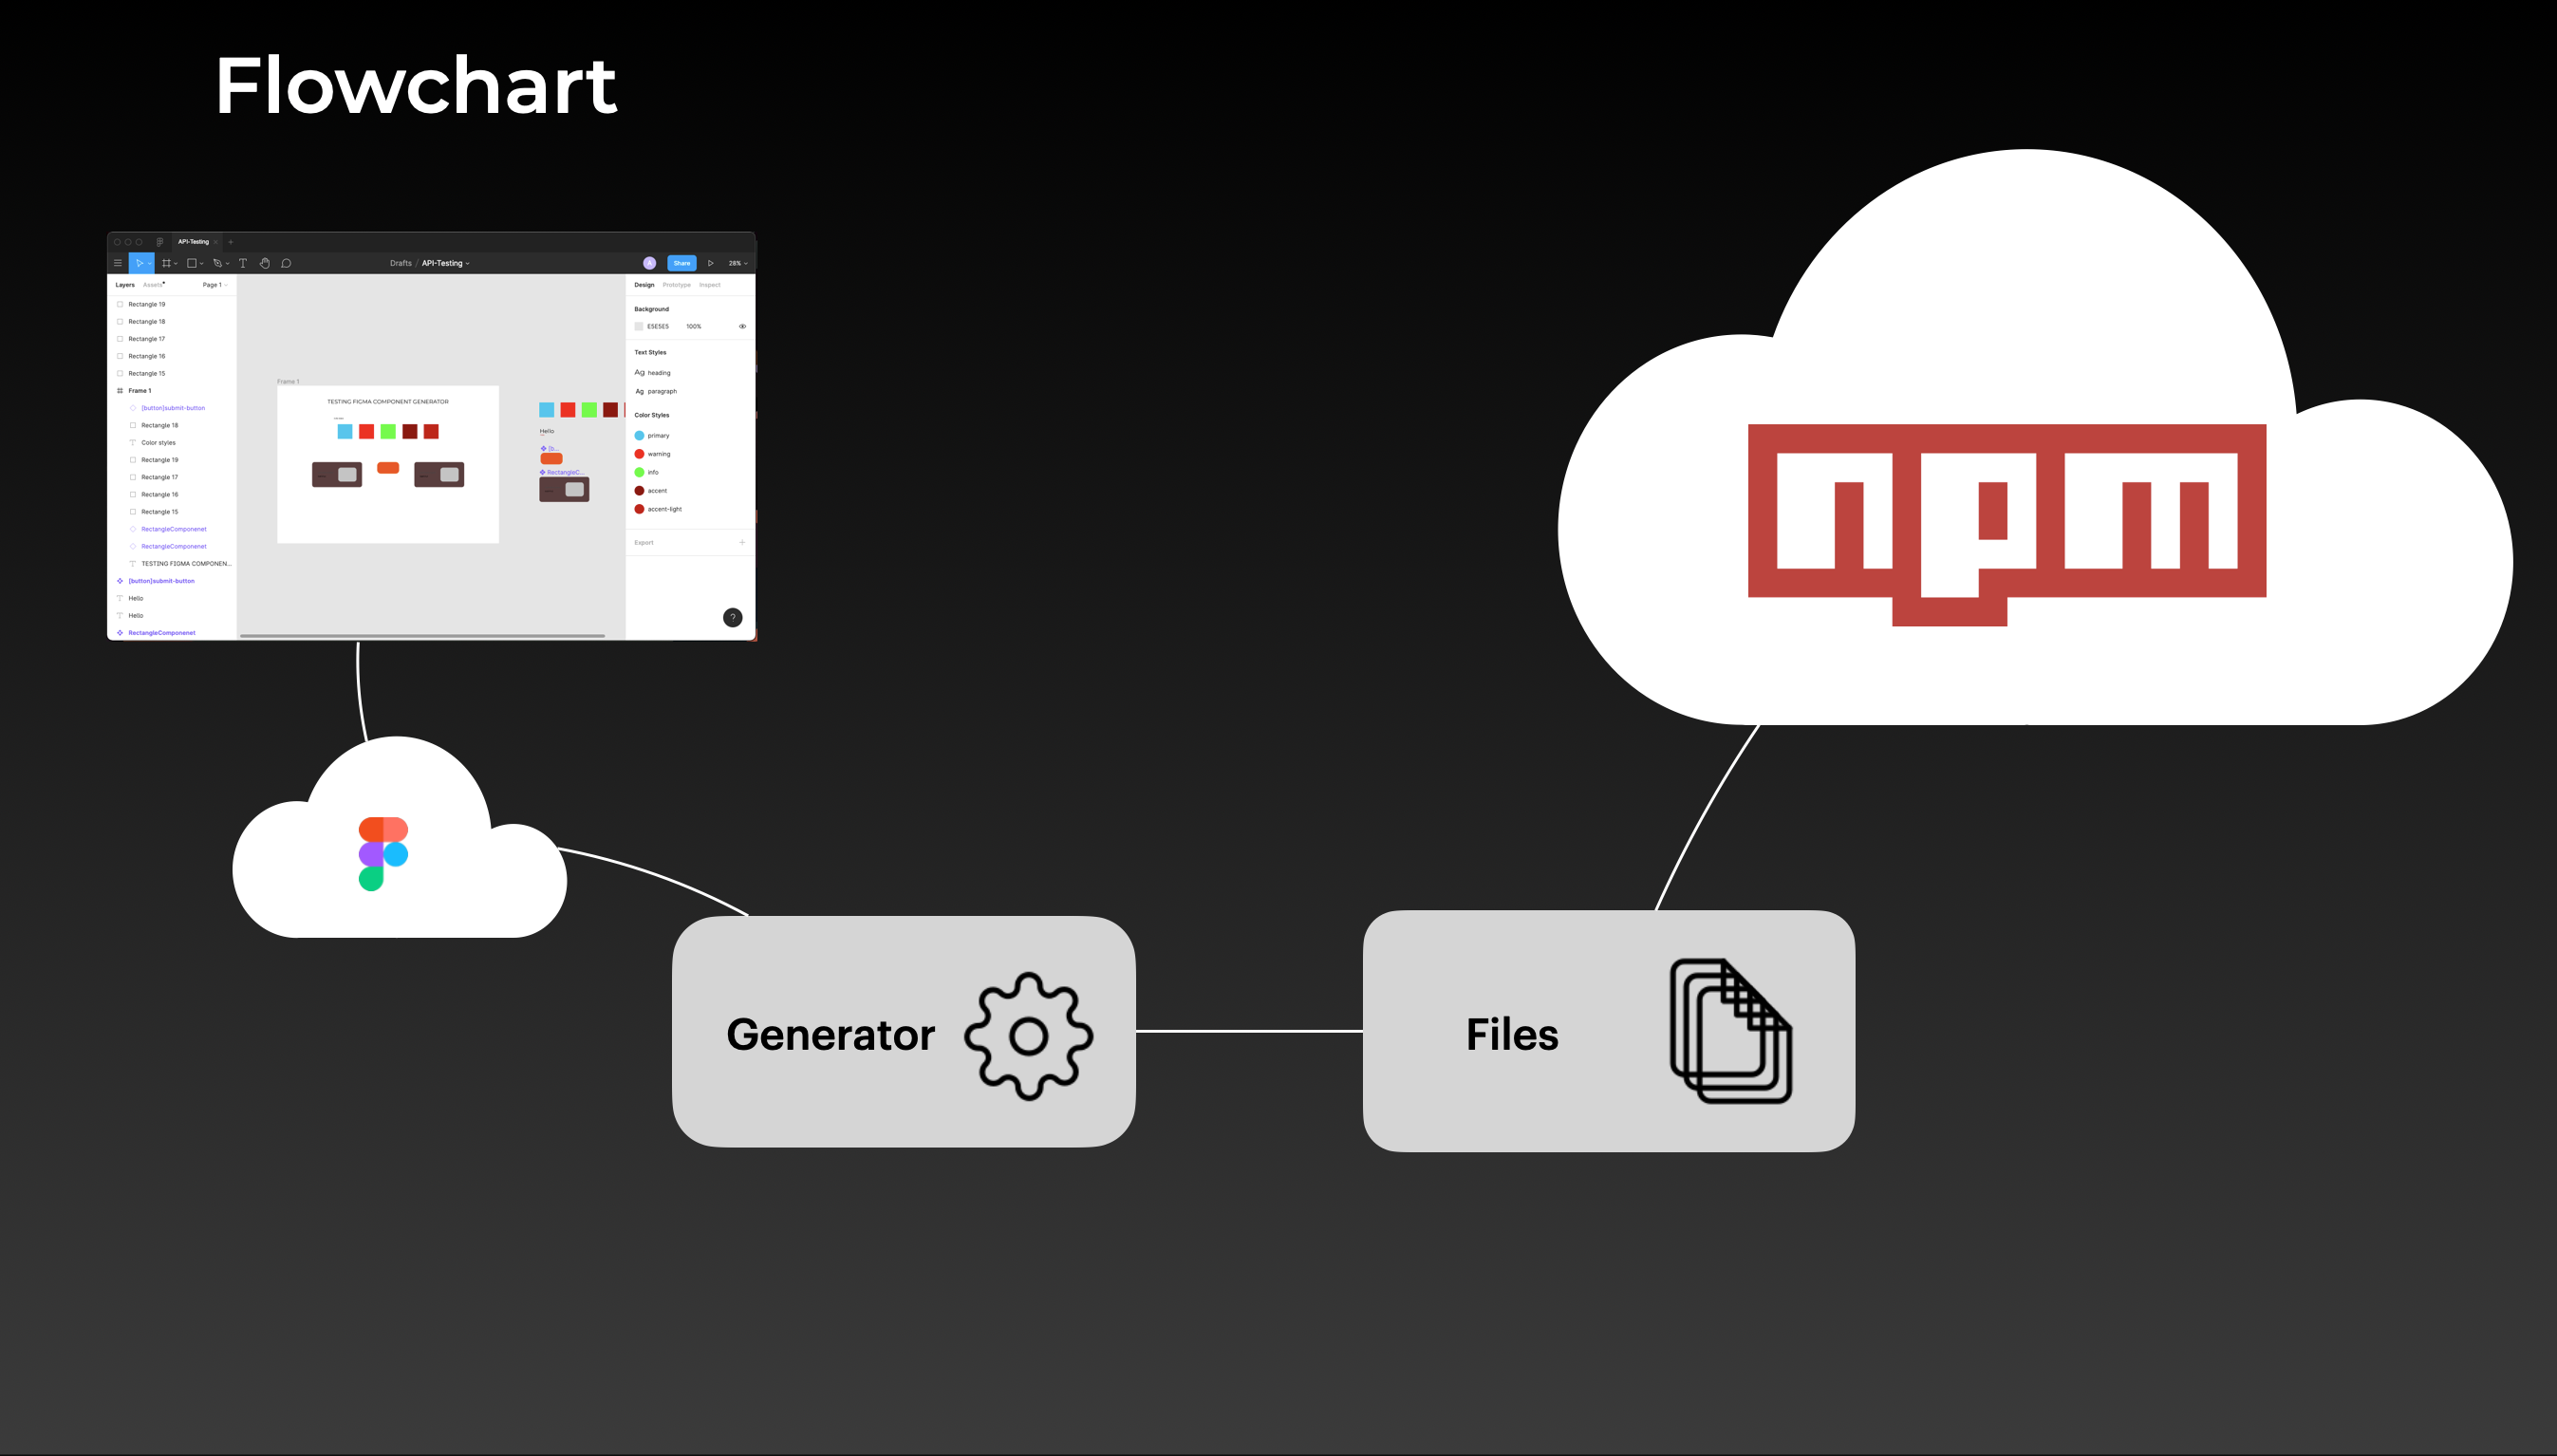
\includegraphics[width=0.8\linewidth]{images/flow.png}
  \caption{Flowchart for data flow in the system. \todo{Bättre bild på g.}}%
  \label{fig:flow}
\end{figure}




\subsection{Competitors}%
\label{sub:Competitors}
The idea of making a design program generate functional code is not new. To get inspired and understand how these software work, we will look at two competitors in this field. 

\subsubsection{Webflow}
Webflow was founded in 2013 and is a product of the famous Y Combinator program. Webflow allows the user to design, create and publish a website all from their web application. Webflow is a visual editing tool. The user does not need to know how to program since Webflow generates HTML, CSS, and JavaScript from the design. Most UI applications let the user move elements freely around the canvas. Webflow is a more static build tool where the elements in the design \textit{snap} in place. Most of the design is made through the control panel, which can be seen in figure \ref{fig:webflow}, and not on the canvas itself \cite{ResponsiveWebDesign}. 

\begin{figure}[H]
  \centering
  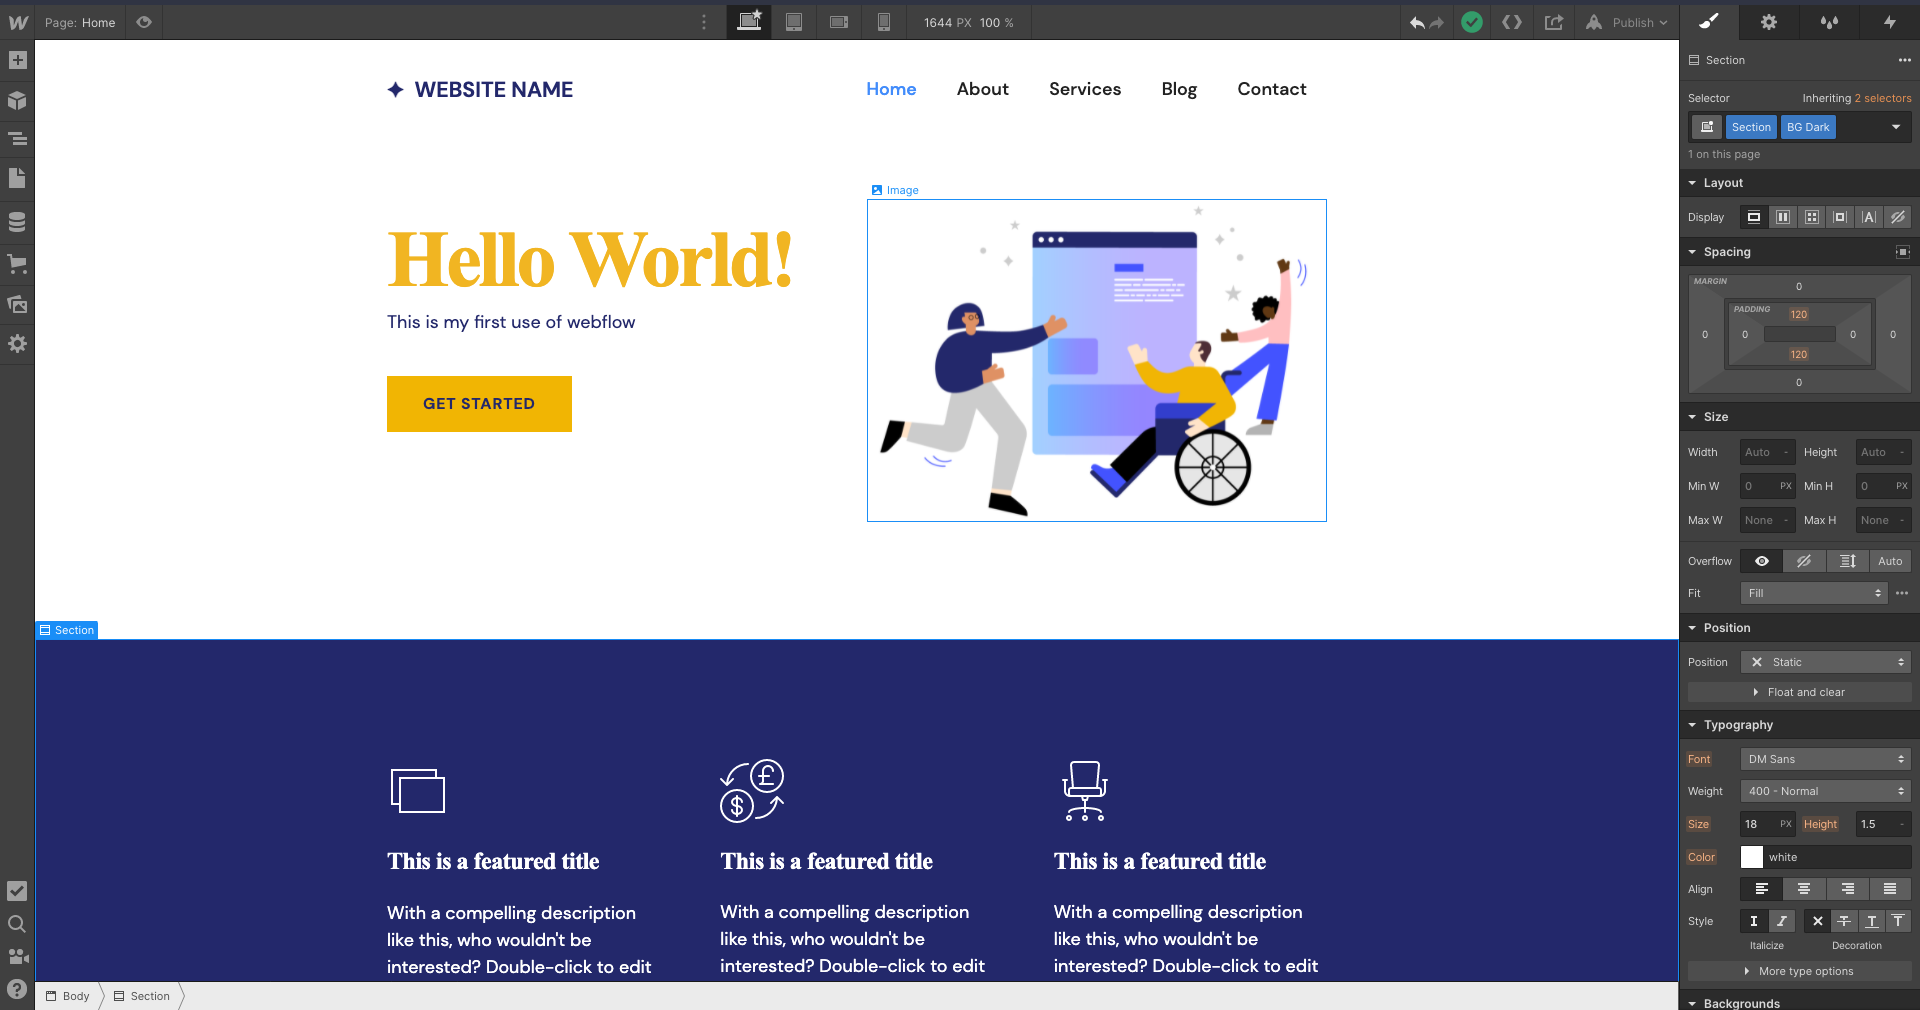
\includegraphics[width=0.8\linewidth]{images/webflow.png}
  \caption{Screenshot of Webflows UI}%
  \label{fig:webflow}
\end{figure}

\subsubsection{Visly}%
\label{ssub:Visly}
Visly was founded in 2018 and is very similar to Figma in how the user designs the product. Visly uses the design to create React components \cite{facebookincReactJavaScriptLibrary}. React is a component-based JavaScript framework made by Facebook. Visly essentially makes it possible to create these components visually. 

\begin{figure}[H]
  \centering
  \includegraphics[width=0.8\linewidth]{images/visly.png}
  \caption{ Screenshot of Vislys UI }%
  \label{fig:visly}
\end{figure}



% \subsubsection{Bravo}%
% \label{ssub:Bravo}

% Build Native IOS och Android apps with Figma. Think this can be the closest to the what I'm trying to do. 



\subsubsection{Competitors summery}%
\label{ssub:Comparison}
Visly and Webflow generate functional code from a graphical user interface (GUI) but in very separate ways. Webflow's service does not require experience with software development, whereas Visly does. Webflow places all functionality in the GUI, which becomes very extensive. Visly, on the other hand, requires the user to know software development and can therefore have a sleek and straightforward GUI.

The disadvantages of both of these competitors are that they are locked with either a framework or software. This dependency is something that we want to avoid as far as possible because of the reason, stated in section \ref{ssub:Knowit Initial Requirements}, that Knowit wants to use the software in all projects. Knowit uses the UI program Figma when designing UI's for their projects. Knowit is happy with the functionality within Figma and does not want to change the software. Therefore the prototype was built around Figma as a UI design platform. 



